\subsubsection{2.3.1.11 Open MPI for Exascale (OMPI-X)}\label{subsubsect:openmpi}

%% {\itshape

%% 	\begin{enumerate}
%% 	\item Rename this file to your project WBS-projectname.tex, for example 2.3.3.01-XSDK4ECP.tex.
%% 	\item Complete this template for your project.  Limit your text to two pages, not counting citations.
%% 	\item Please avoid changing the content of main.tex.
%% 	\item Put any references in a .bib file with the same root name, for example 2.3.3.01-XSDK4ECP.bib.
%% 	\item Remember to include any image files you reference in your text.
%%     \item The files 2.3.3.01-XSDK4ECP.tex, 2.3.3.01-XSDK4ECP.bib and xSDK-diagram.jpeg are included as examples for your reference.  You can remove them from what you upload.
%% 	\end{enumerate}
%% }

\paragraph{Overview}
%% \textit{Provide an overview of your project.  You might find that the introductory text from your Fall 2017 Project Summary \url{https://confluence.exascaleproject.org/display/1ST/Fall+2017+ECP+ST+Project+Summaries} useful as a starting draft.}

The OMPI-X project ensures that the Message Passing Interface (MPI)
standard, and its specific implementation in Open MPI meet the needs
of the ECP community in terms of performance, scalability, and
capabilities or features. MPI is the predominant interface for
inter-process communication in high-end computing.  Nearly all of the
ECP application (AD) projects (93\%~\cite{Bernholdt:2017:smu-talk})
and the majority of software technology (ST) projects
(57\%~\cite{Bernholdt:2017:smu-talk}) rely on it.
%% Since its
%% inception, the MPI standard has evolved to address the changing needs
%% of massively parallel libraries and applications as well as the
%% systems on which they are run.
With the impending exascale era, the
pace of change and growing diversity of HPC architectures pose new
challenges that the MPI standard must address.  The OMPI-X project is
active in the MPI Forum standards organization, and works within it to
raise and resolve key issues facing ECP applications and libraries.

Open MPI is an open source, community-based implementation of the MPI
standard that is
%% freely available, and
used by a number of prominent
HPC vendors as the basis for their commercial MPI offerings.  The
OMPI-X team is comprised of active members of the Open MPI community,
with an extensive history of contributions to this community.
%% the development and
%% maintenance of the library.
The OMPI-X project focuses on prototyping
and demonstrating exascale-relevant proposals under consideration by
the MPI Forum, as well as improving the fundamental performance and
scalability of Open MPI, particularly for exascale-relevant platforms
and job sizes.  MPI users will be able to take advantage of these
enhancements simply by linking against recent builds of the Open MPI
library.

Without the OMPI-X project, there will be less competition and less
innovation in addressing the needs of ECP users in the critical area
of scalable, performant, and capable exascale-quality inter-process
communication capabilities.

\paragraph{Key  Challenges}
%% \textit{Describe what is hard to do, why it is challenging.}
A number of aspects of ``exascale'' levels
of computing pose serious challenges to the ``tried and true'' message
passing model presented by MPI and its implementations, including Open
MPI.
%
Keeping pace with changes in HPC architecture is a major challenge.
The MPI ecosystem (the standard and its implementations) needs to
evolve to address challenges
%% on the programming side
driven by
architectural change, as well taking advantage of new features and
capabilities.
%
As applications and libraries
%% they rely on
build up to exascale,
%% levels of computing and beyond,
the number of node, processes, and
threads required will rise significantly, whereas other key resources,
such as memory tend to go \emph{down} on a per-node, -process, or
-thread basis.  This emphasizes the importance of scalability in terms
of both performance and resource utilization.
%% to allow MPI to scale to
%% meet those needs.
%
Finally, we must work with in the much larger and broader MPI
community to find approaches to address these challenges which do not
adversely impact the capabilities, performance, or scalability for
other users of MPI and Open MPI.

\paragraph{Solution Strategy}
%% \textit{Describe your basic strategy for addressing the challenges.}
The OMPI-X project is working across a number of fronts to address
these challenges.

\emph{Runtime Interoperability for MPI+X and Beyond} MPI is
increasingly being used concurrently with other runtime environments.
This includes both ``MPI+X'' approaches, where X
%% , in the ECP
%% environment, X
is most often a threading model, such as OpenMP, as
well as the use of multiple inter-process runtimes within a single
application.  Concerns include awareness of other runtimes,
cooperative resource management capabilities, and ensuring that all
concurrently active runtimes make progress.  We will develop APIs and
demonstrate capabilities for interoperability in both MPI+X and
multiple inter-process runtime situations.

\emph{Extending the MPI Standard to Better Support Exascale
Architectures} The MPI community is considering for standardization a
number of ideas that 
%% A number of ideas under consideration by the MPI
%% community for standardization
are particularly important to supporting
the architectural and system size characteristics anticipated for
exascale.  ``Finepoints'' and ``Endpoints''
%% are approaches to
deal
with the growing use of threading for node-level concurrency, in
combination with MPI.  ``Sessions'' increases the flexibility of MPI
semantics in a number of areas, which in turn can open opportunities
for enhanced scalability, as well as easier support for
multi-component applications such as coupled multi-physics
simulations.  We will develop prototype implementations and work with
ECP teams to evaluate the ability of these approaches to address ECP
requirements in order to facilitate the standardization process.

\emph{Open MPI Scalability and Performance} As we push the scale of
both hardware and applications, we stress MPI implementations and
expose areas that need to be improved in order to improve scalability.
OMPI-X is targeting memory usage within Open MPI, as well as remote
memory access (RMA), tag matching, and other areas, for improvements
in both scalability and performance.

\emph{Supporting More Dynamic Execution Environments} We are
developing and implementing strategies to help MPI applications
better deal with topological process layout preferences
%% as well as
%% responding to
and contention in the network.

\emph{Resilience in MPI and Open MPI} Concerns about system and
application resilience increase as either scales in size.
%% (number of
%% components or MPI ranks).
We will provide implementations of the
User-Level Fault Mitigation (ULFM) and ReInit proposals currently
under discussion within the MPI Forum, as well as demonstrations of
their use, in order to help drive standardization discussions, and to
help ECP team understand how they can take advantage of these
capabilities to improve the resilience of their libraries and
applications.

\emph{MPI Tools Interfaces}  Several interfaces within the
MPI standard are primarily used to support performance and
correctness tools.
%% of various kinds.
The MPI Forum is in the process
of making significant revisions and extensions to these interfaces.
We will track the discussions in the Forum and provide prototype
implementations within Open MPI to facilitate evaluation and provide
feedback.
%% on the standardization discussions.
We will work with the
ECP community, including tool developers, to make additional data
available through the MPI\_T interface.

\emph{Quality Assurance for Open MPI}  We are enhancing the
Open MPI testing infrastructure, adding tests to reflect ECP
requirements, and instantiating routine testing on systems of
importance to ECP.

\paragraph{Recent Progress}
%% \textit{Describe what you have done recently.  It would be good to
%% have some kind of figure or diagram in this section.}
One of the first activities of the project was to conduct a survey of
ECP AD and ST projects to better understand their current and expected
usage of MPI, and look for significant issues in the MPI environment
that we might have overlooked in our planning for the project.  A
paper describing the survey results was presented at the ExaMPI 2017
workshop held in conjunction with SC17~\cite{Bernholdt:2017:smu-talk},
and will appear in a special issue of Concurrency and Computing:
Practice and Experience.  The survey has generated a great deal of
interest in the MPI community, and there are plans to expand the scope
to provide a better characterization of MPI usage around the world.

We have delivered an implementation of the User-Level Fault Mitigation
(ULFM) resilience approach, which are under consideration by the MPI
Forum for inclusion in the standard.  ULFM provides the basic building
blocks for cheap, tailored recovery capabilities within applications
and libraries using MPI.  ULFM imposes no overhead on raw
communication performance on ECP-relevant hardware.  We are now
working with several application teams to demonstrate the capabilities
it provides.

\begin{wrapfigure}{r}{4in}
\begin{minipage}[c]{2in}
\vspace{0pt}
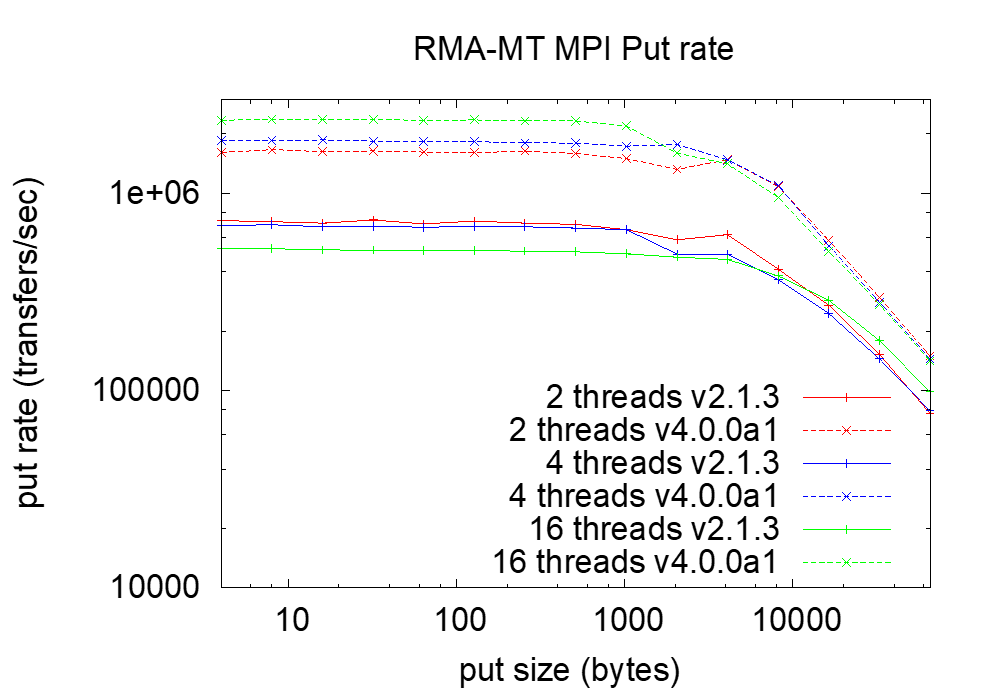
\includegraphics[width=\textwidth]{projects/2.3.1-PMR/2.3.1.11-OMPI-X/pritchard-rma-mt-put-rate.png}
\end{minipage}
\begin{minipage}[c]{2in}
\vspace{0pt}
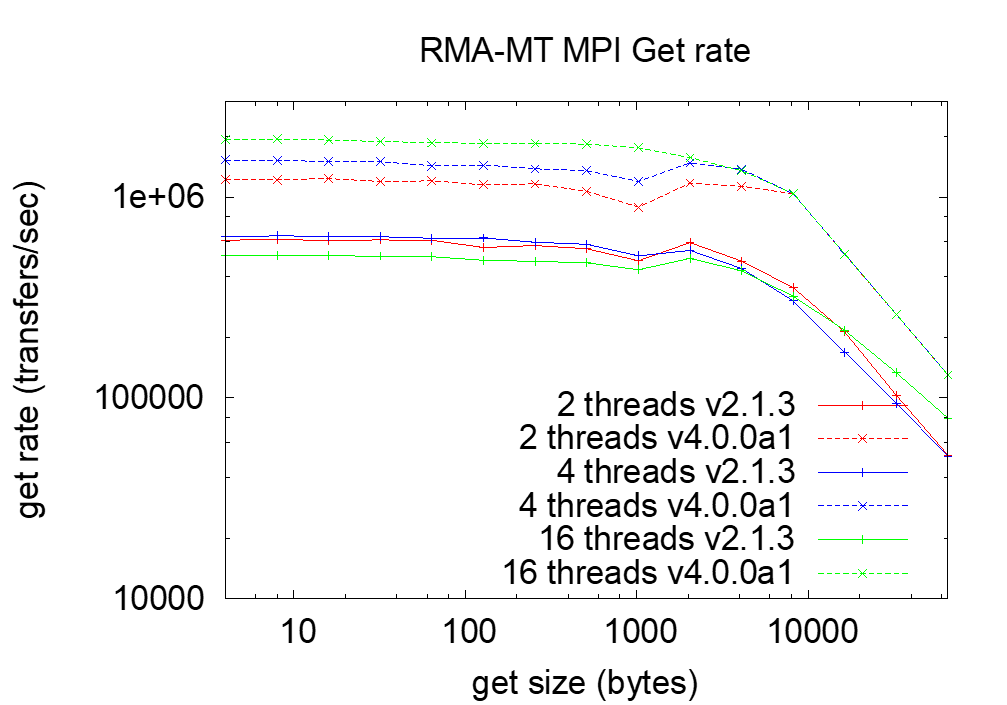
\includegraphics[width=\textwidth]{projects/2.3.1-PMR/2.3.1.11-OMPI-X/pritchard-rma-mt-get-rate.png}
\end{minipage}
\caption{Comparison of put (left) and get (right) RMA performance in a
multi-threaded context for Open MPI.  Recent OMPI-X contributions are
reflected in version 4.0.0a1 (top group of lines), in comparison with
v2.1.3.}
\label{fig:ompix-rma}
\end{wrapfigure}

We expect to be working on scalability and performance of Open MPI
throughout the project, but some early successes have been
demonstrated.  We have improved the RMA implementation so achieve
performance levels comparable to those obtained only by high tuned
implementations by vendors and significantly improved their
performance in multi-threaded contexts (Fig.~\ref{fig:ompix-rma}).  We
have also been able to improve message matching by up to 2$\times$
generally, and up to 45$\times$ on Intel Xeon Phi processors, and we
have made significant improvement to performance when MPI is used in a
multi-threaded environment.

Early work with the prototype implementation of Finepoints shows
improvements of 25\% in communication costs and 5\% in overall
execution time for one ECP mini-app.
%
Open MPI support for the MPI\_T interface has been extended~\cite{icl:957} to
provide a set of low-level counters to present a more detailed performance
characteristics map to tools and to users.
%
Finally, we have deployed the MTT testing infrastructure used by Open
MPI on ORNL's SummitDev and Summit platforms, as well as improving the
MTT system itself.

\paragraph{Next Steps}
%% \textit{Describe what you are working on next.}
We are making progress across multiple fronts, some of which has been
described above.  In FY18, we expect to complete our primary efforts
in the area of resilience in Open MPI, an implementation of the
``ReInit'' approach to complement the already completed User-Level
Fault Mitigation (ULFM) capability.  Both approaches continue to be
debated within the MPI Forum, but we are hopeful that demonstrations
based on our implementations can help bring these discussions to a
conclusion. Early in FY19, we will also be delivering a formal
proposal and prototype implementation of the ``Finepoints'' approach to
supporting environments with large numbers of threads.
